\documentclass[runningheads,anonymous]{llncs}

\usepackage{graphicx}
\newcommand{\SWAT}{SWAF}
\usepackage{graphicx}
\usepackage{listings}
\usepackage{subfig}
\usepackage[utf8]{inputenc}


\begin{document}

\title{An End-User Semantic Web Augmentation tool}

\author{Cristian Sottile\inst{1,2} \and
Sergio Firmenich\inst{1,3} \and
Diego Torres\inst{1,2,3}}

\authorrunning{C. Sottile et al.}

\institute{LIFIA, Facultad de Informática, UNLP, Argentina \and
Comisión de Investigaciones Científicas de la Provincia de Buenos
Aires, Argentina \and
Consejo Nacional de Investigaciones Científicas y Técnicas, Argentina \and
Departamento de Ciencia y Tecnología, UNQ, Argentina}

\maketitle

\begin{abstract}
    Web Augmentation is usually applied to add, remove and change Web sites' functionalities, content, and presentation. Content-based Web Augmentation is commonly performed by integrating content from an external Web site into the current one. In this article, we explore the use of the Semantic Web as a source of information to be incorporated to any Web site, aiming to simplify the development of Web Augmentation based on Semantic Web data. Our approach allows end-users without any programming skills to build Web Augmentation scripts that takes some information from the current Web page, and produce new related information gathered from the Semantic Web. This article introduces a pipeline process for building SWA and an End-User Development tool called SWAX to create augmentation layers without the need for any programming or SW skills.

\keywords{Semantic Web \and Web Augmentation \and User Interface}
\end{abstract}

\section{Introduction}
\label{sec-introduction}

The Semantic Web \cite{Berners-Lee2001TheWeb,Shadbolt2006TheRevisited} (SW) provides sources of semantic information useful to be interchanged among computer systems with a standard model called RDF. Most of RDF data sources allow being queried through a SPARQL endpoint.

Web Augmentation (WA) is an approach to improve Web applications by incorporing new functionalities.  A common strategy is to enhance them on the client side \cite{Bouvin1999UnifyingAugmentation}, after it is received from the server.

Semantic Web Augmentation (SWA) is a particular type of WA where the SW provides the new information. The SW is accessed via a SPARQL endpoint or RDF API to extract information pieces, which are then adapted and inserted into the DOM structure on the client side. The Website ends up including the original contents plus the new ones from the SW. In this article we tackle with a kind of SWA where the new information is related to the content of the Website. SWA developers need to be skilled in client-side and SW technologies \cite{Rico2012AData}.

This article introduces both a pipeline process for building SWA and an End-User Development tool called SWAX to create augmentation layers without the need for any programming or SW skills.

Section \ref{sec-process} describes the pipeline process for building SWA. Section \ref{sec-tool} introduces the End-User development tool designed as a Web Browser extension. Related work is analyzed in Section \ref{sec-related_work}, and Section \ref{sec-conclusions} details conclusions and further work. 


\section{The process}
\label{sec-process}

This section explains the process for building SWA. It is a pipeline process where each component receives as input the output of its predecessor, and consists of three main steps:
\begin{itemize}
  \item \textbf{Data extration:} We stated that our kind of SWA will involve the information present in the desired Website. In this step, these data are extracted from the DOM.
  
  \item \textbf{Data fetching:} Given a generic SPARQL query and the \textit{extracted data}, this step fills the generic query with the data, producing a specific query for each one, and then run these queries against a SPARQL endpoint, obtaining new information from the Semantic Web.
  
  \item \textbf{Insertion:} Given an HTML template and the \textit{fetched data}, this steps generates specific HTML elements by filling the templates with the data, and inserts them in the Website, performing the Web Augmentation.
\end{itemize}
  
  
\section{An End-User Development Tool for SWA}
\label{sec-tool}

This section introduces an End-User Development Tool for building SWA, which we call SWAX\footnote{Source code and video-tutorials at \url{https://github.com/cfsottile/swa-extension}}. It is a Web browser extension whose functionality is based upon the process described in Section \ref{sec-process}, and allows to build a WA script based on the current Website. It can be enabled in any Web page, initiating a wizard-like UI to configure the augmentation in a sequence of intuitive steps. The result is a script that is general enough to augment all Web pages whose DOM structure and semantics are similar to the original one. One configuration, several executions. Additionally, the script can be executed to test its results.

As a guide example, we will take the IMDb\footnote{IMDb stands for Internet Movie Database. \url{http://imdb.com}} website, and we will aim to improve the films Websites by adding the amount of Oscars every cast member won. The \textit{``The Godfather II''} page on IMDb\footnote{\url{https://www.imdb.com/title/tt0071562/}} could be used to produce a script to augment this and every IMDb film page. In the following, we introduce the tool's sequence of steps using this example.

\begin{enumerate}
  \item \textbf{Extraction:} First, the user selects what DOM elements from the Web page will be used as data input in the semantic augmentation, by enabling the selection mode and clicking them. Continuing with our example, these would be actor's and actress' names. Then, the user defines how to extract the information contained in the selected DOM element (e.g., the text content or the HREF) and the tool shows the \textit{value} extracted from it.
  
  \item \textbf{Querying:} The semantic query that will retrieve the new information from the SW must be defined. There are different mechanisms to help the SPARQL query building with visual tools. We delegate it to Visual SPARQL Builder (VSB) \cite{mci/Eipert2015}, which provides an intuitive interface to assist users in vocabulary and properties detection.
  Our tool provides an augmentation layer also on VSB for communication purposes. The resulting SPARQL query will be executed against the DBpedia SPARQL endpoint, obtaining the augmentation data.

  \item \textbf{Building:} This step involves the definition of the HTML template that will be used to insert the augmentation data to the Web page. The user must write the HTML code including references to the augmentation data; however, the template may consist of only references, thus not being mandatory for the user to know any HTML. References to augmentation data are presented as buttons that, when clicked, insert the reference into the template input.
  
  \item \textbf{Insertion:} This step configures the weaving of the HTML augmentation elements built in the previous step. The user must choose the wanted places in the Web page to inject them. This is done similarly to the Selection step, by selecting HTML elements from the DOM.
  
  \item \textbf{Saving:} The user will define a set of URLs where the augmentation should be applied. In our cast example, this would be \texttt{https://www.imdb.com/title/*}. Then, the user can \textit{save} the augmentation script, which will be applied every time a URL within the set is opened, or \textit{try} it in the current page for testing purposes. Figure \ref{fig-oscars} shows the cast section of the \textit{``The Godfather II''} page before and after the augmentation.
\end{enumerate}

\begin{figure}
  \centering
    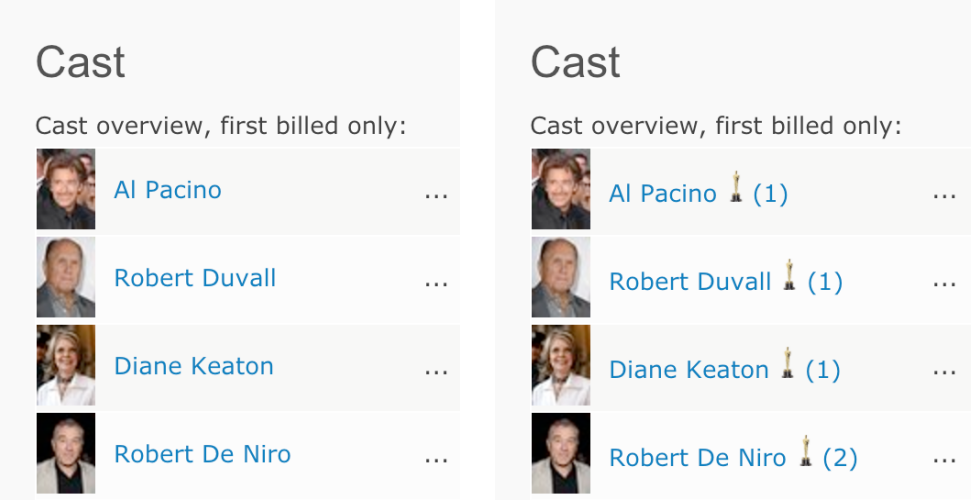
\includegraphics[width=0.7\linewidth]{oscars.png}
    \caption{Case study: Oscars}
    \label{fig-oscars}
\end{figure}

\section{Related Work}
\label{sec-related_work}
Rico et al. \cite{Rico2012AData} introduced a tool to allow Web developers with no SW skills to create templates capable of handling semantic data. 
WOA \cite{DBLP:conf/icwe/FirmenichBRWB16} presents an approach for the creation of WA layers by firstly annotating Web contents with semantic tags. 
Most SW improvements of non-SW applications are based on the \textit{semantification} of Web pages from social efforts \cite{torres2011semdrops,annoteawww10}. 
For the best of our knowledge, there exist no end-user tools for defining the weaving of information extracted from the SW in the current context of Web browsing.
 
\section{Conclusions and Further Work}
\label{sec-conclusions}


The SW is in a mature state since many years. However, it is not common to see tools for allowing Web users communities to consume all this infrastructure. In this paper, we present a pipeline processs for building SWA, and an End-User Development tool based upon it called SWAX to create augmentation layers. The approach allows end-users without any programming skills to produce generic WA scripts that allow for enriching the contents of groups of Web pages.

The first future work is the need for an exhaustive evaluation. The prominent prototype demonstrated well behavior and easy to use augmentation tasks in laboratory tests. Nonetheless, we are designing usability tests with a group of developers. Additionally, more extraction and insertion strategies are in development, as well as user experience improvements. Also, there are several SPARQL query builders like VSB that could be adapted for SWAX.


\bibliographystyle{splncs04}
\bibliography{biblio}
\end{document}
